\section{Performance Evaluation}
\label{sec:evaluation}

We evaluate ASZ in terms of rate--distortion performance, total runtime across error bounds with per-file tuning, and plan reuse across related files.

\subsection{Experimental Setup}
\label{sec:evaluation:setup}

\subsubsection{Evaluation Platform}

We conduct all experiments on Purdue Anvil. Each standard compute node contains two 64-core AMD EPYC 7763 processors and 235~GiB of memory available to jobs. Every codec execution uses one physical CPU core. We compile ASZ with GCC 11.2.0 using \verb|-Ofast -march=native -mavx2 -mfma|.

\subsubsection{Scientific Datasets}

Table~\ref{tab:evaluation-datasets} summarizes the 18 fields used in the rate--distortion and runtime experiments. They span weather and climate data, seismic imaging, fluid dynamics, cosmology, electronic-structure calculations, hydrodynamics, and X-ray experiments. For the plan-transfer experiments in Section~\ref{sec:evaluation:transfer}, we use related time steps or fields from data sources represented in Table~\ref{tab:evaluation-datasets}.

\begin{table*}[htb]
    \centering
    \caption{Scientific fields used in the evaluation.}
    \label{tab:evaluation-datasets}
    \footnotesize
    \setlength{\tabcolsep}{3pt}
    \begin{tabular}{@{}lll lr@{\hspace{0.8em}}|@{\hspace{0.8em}}lll lr@{}}
        \toprule
        \textbf{Dataset} & \textbf{Field} & \textbf{Index} & \textbf{Domain} & \textbf{Size} &
        \textbf{Dataset} & \textbf{Field} & \textbf{Index} & \textbf{Domain} & \textbf{Size} \\
        \midrule
        QMCPACK & Orbital & 144 & Electronic structure & 2.09~MiB & FLASH & Density & 22 & Hydrodynamics & 32.00~MiB \\
        APS & Kaz & -- & X-ray & 62.38~MiB & Isabel & PRECIP & 24 & Weather & 95.37~MiB \\
        Isabel & QGRAUP & 24 & Weather & 95.37~MiB & Miranda & Velocity-$x$ & -- & Fluid & 144.00~MiB \\
        Miranda & Velocity-$z$ & -- & Fluid & 144.00~MiB & RTM Small & -- & 0360 & Seismic & 180.73~MiB \\
        Aramco & -- & 1800 & Seismic & 180.73~MiB & SCALE-LETKF & PRES & -- & Weather & 538.33~MiB \\
        SCALE-LETKF & T & -- & Weather & 538.33~MiB & CESM & VD01 & 31 & Climate & 642.70~MiB \\
        CESM & UU & 31 & Climate & 642.70~MiB & APS CSSI & -- & L0471 & X-ray & 1.35~GiB \\
        Nyx & Baryon density & 632 & Cosmology & 4.00~GiB & Nyx & Temperature & 632 & Cosmology & 4.00~GiB \\
        APSU & -- & 004 & X-ray & 10.78~GiB & APSU & -- & 006 & X-ray & 43.10~GiB \\
        \bottomrule
    \end{tabular}
\end{table*}

\subsubsection{Baselines and Metrics}

We compare ASZ with two groups of scientific lossy compressors. SZ3, QoZ, and ZFP form the high-performance group, covering prediction-based and block-transform methods. SPERR serves as a high-ratio wavelet-based baseline.

\subsection{Rate--Distortion Performance}
\label{sec:evaluation:rd}

Figure~\ref{fig:evaluation-rd} compares the full RD curves. We summarize each comparison over the common PSNR range as a compression-ratio gain. Across the 18 fields, ASZ achieves geometric-mean compression ratios that are $2.48\times$, $2.07\times$, $6.18\times$, and $1.36\times$ those of SZ3, QoZ, ZFP, and SPERR, respectively. ASZ outperforms SZ3, QoZ, and ZFP on all 18 fields and SPERR on 10 fields.

ASZ improves on SZ3 and QoZ by adapting both prediction and lossless coding at finer granularity. Its unrestricted per-round axis choices can repeatedly use the direction that best matches the correlations at the current reference spacings. For 1D4R, ASZ searches a finer coefficient set within each block than QoZ's predefined one-dimensional formulas, allowing closer adaptation to local correlations. ASZ also selects a QB serialization order for every round, placing strongly correlated QBs consecutively before Huffman encoding and Zstd. These choices reduce prediction residuals and make the QB stream more compressible.

SPERR comes closest to ASZ because both methods perform multiscale spatial decorrelation. ASZ's coarse-to-fine interpolation converts the directional correlations selected in each round into prediction residuals. SPERR instead uses a fixed multilevel three-dimensional CDF 9/7 transform that recursively processes all three axes, exploiting spatial coherence across multiple scales and compacting information into wavelet coefficients. However, this shared principle does not give SPERR ASZ's data-dependent adaptation. SPERR uses a fixed transform rather than selecting the prediction axis and coefficients for each round or block. Its pointwise error guarantee also requires a separate stream of corrections for reconstructed values that exceed the error bound. These differences help explain why ASZ attains a $1.36\times$ geometric-mean compression-ratio advantage and outperforms SPERR on 10 of the 18 fields. SPERR's codec time is also higher because it performs the multilevel transform, repeatedly traverses coefficient bit planes, and applies an inverse transform to locate outliers within each large three-dimensional chunk. The \texttt{sperr3d} default used in our experiments sets the preferred chunk size to $256^3$ values. Section~\ref{sec:evaluation:codec-time} quantifies this time difference.

\begin{figure*}[htb]
    \centering
    \IfFileExists{figs/5/rate-distortion-final-eighteen-log.png}{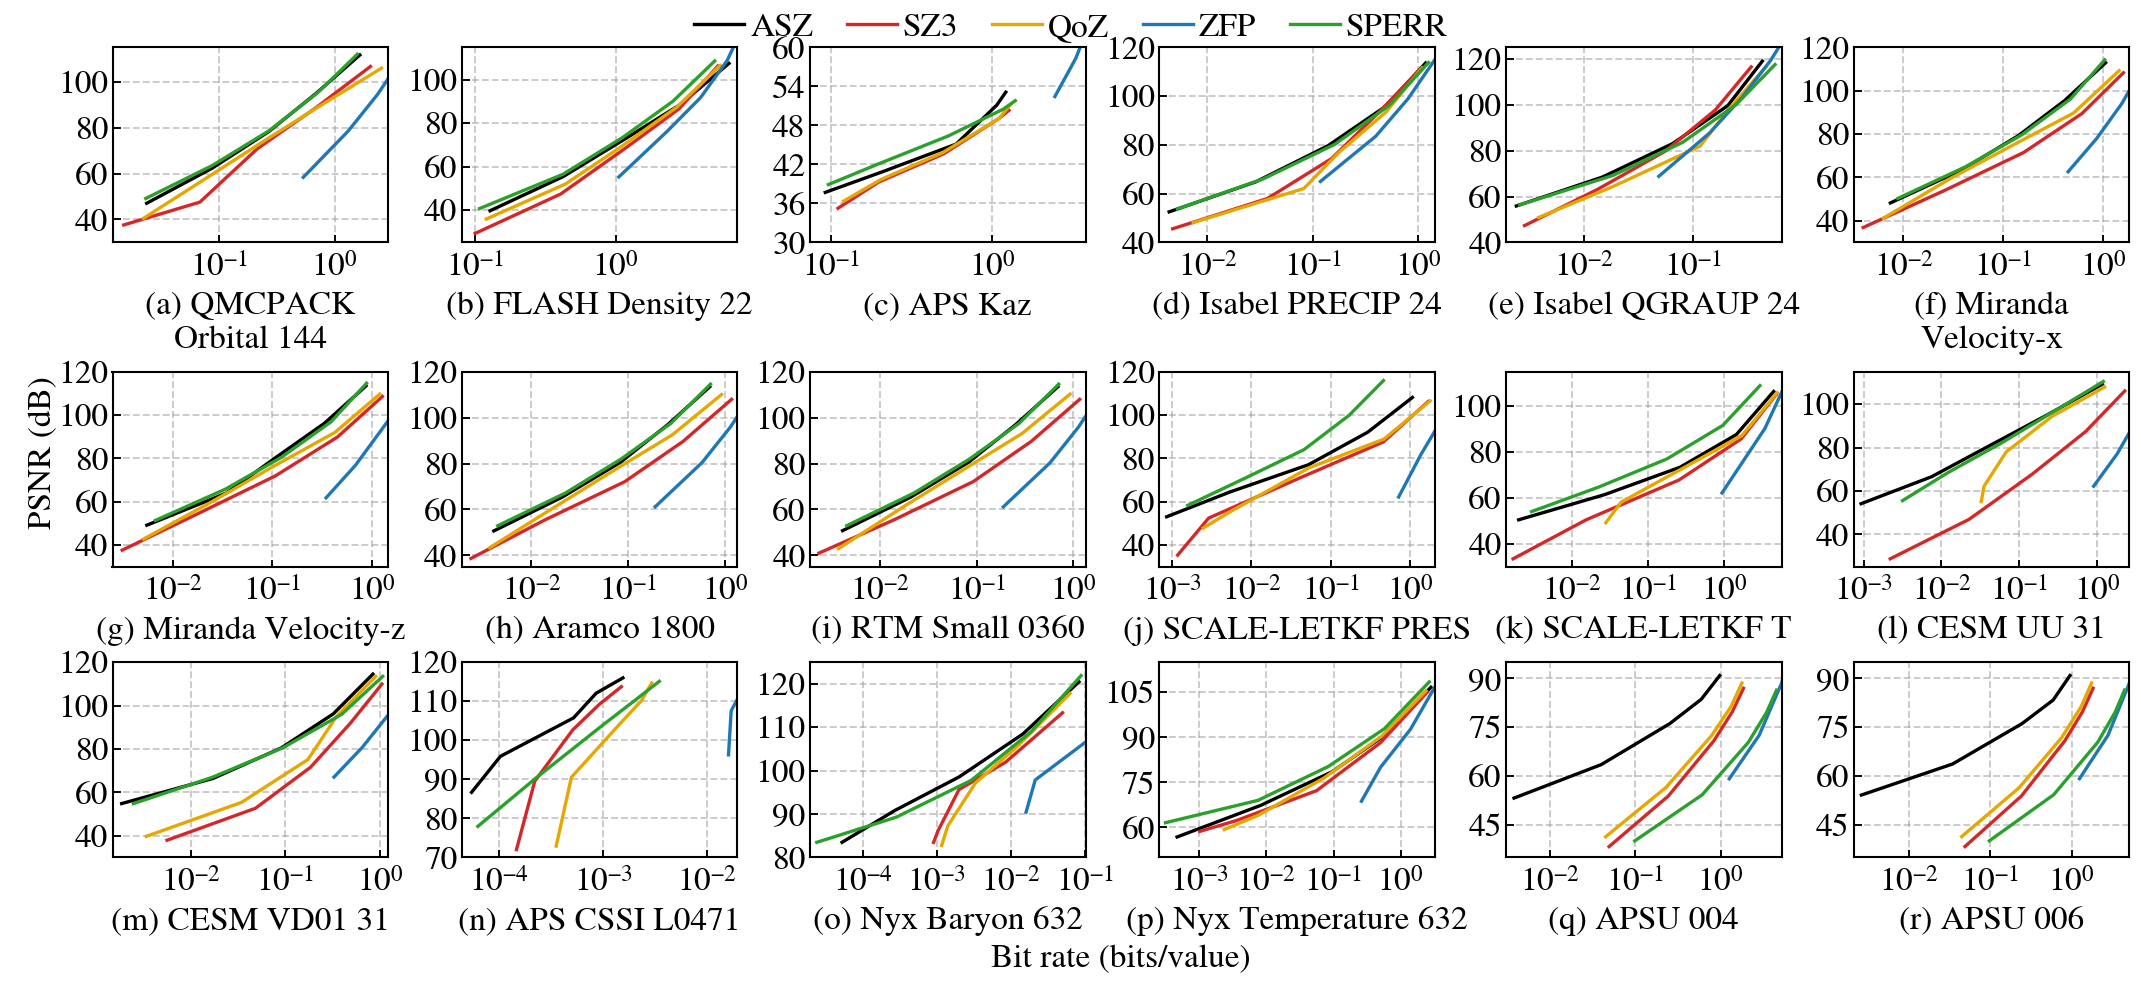
\includegraphics{figs/5/rate-distortion-final-eighteen-log.png}}{\fbox{\parbox[c][1.5in][c]{0.96\textwidth}{\centering Final 18-field rate--distortion figure pending.}}}
    \caption{Rate--distortion performance on 18 scientific fields. At matched PSNR, ASZ achieves $2.48\times$, $2.07\times$, $6.18\times$, and $1.36\times$ the geometric-mean compression ratios of SZ3, QoZ, ZFP, and SPERR, respectively, outperforming the first three on all 18 fields and SPERR on 10.}
    \label{fig:evaluation-rd}
\end{figure*}

\subsection{Total Runtime Across Error Bounds}
\label{sec:evaluation:codec-time}

Figure~\ref{fig:evaluation-codec-time} compares ASZ with SZ3, QoZ, ZFP, and SPERR at all five relative error bounds. Each stacked bar reports the total runtime as the sum of the timed in-memory stages. ASZ includes preprocessing, compression, and decompression, while each baseline includes compression and decompression. File input, file output, and post-run error verification are excluded. ASZ's compression segment includes its data-range scan, and the SZ3 and QoZ compression segments include their built-in tuning. Across the 90 field--error-bound combinations, ASZ's geometric-mean total runtime is $0.81\times$ that of QoZ and $0.43\times$ that of SPERR, and ASZ is faster in 70 and 89 combinations, respectively. Its total runtime is $1.72\times$ that of SZ3 and $2.36\times$ that of ZFP. Considering the timed stages separately, ASZ provides geometric-mean compression and decompression speedups of $1.63\times$ and $1.71\times$ over QoZ and $2.85\times$ and $4.02\times$ over SPERR. At the middle error bound of each field, plan generation accounts for 23.94\% of ASZ's total runtime. These time differences accompany the compression-ratio improvements reported in Section~\ref{sec:evaluation:rd}.

\begin{figure*}[htb]
    \centering
    \IfFileExists{figs/5/time-breakdown-final-eighteen-vs-rel-eb.png}{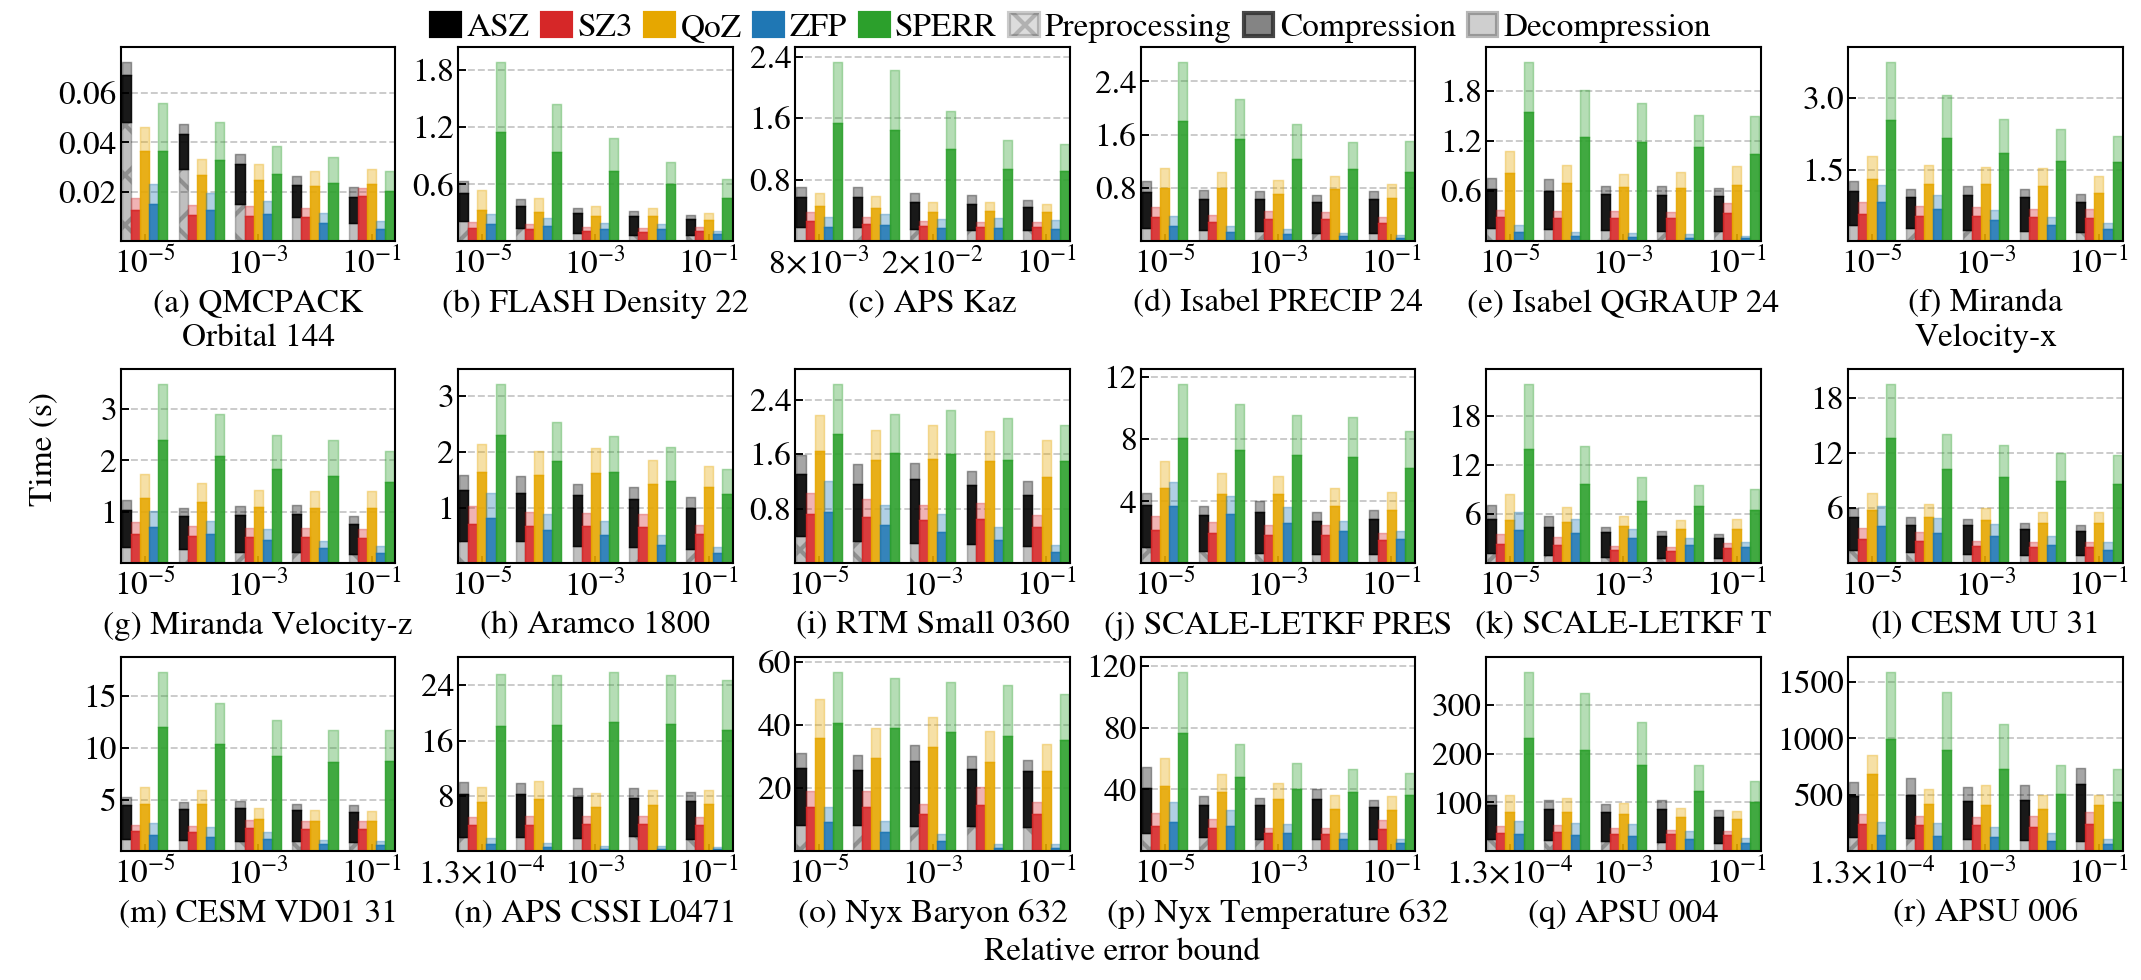
\includegraphics{figs/5/time-breakdown-final-eighteen-vs-rel-eb.png}}{\fbox{\parbox[c][1.5in][c]{0.96\textwidth}{\centering Final 18-field codec-time figure pending.}}}
    \caption{Total runtime across five relative error bounds. Each error-bound group contains one bar per method. ASZ stacks preprocessing, compression, and decompression, while each baseline stacks compression and decompression. ASZ's geometric-mean total runtime is $0.81\times$ that of QoZ and $0.43\times$ that of SPERR.}
    \label{fig:evaluation-codec-time}
\end{figure*}

\subsection{Plan Transferability Across Related Files}
\label{sec:evaluation:transfer}

This subsection evaluates ASZ's ability to reuse a plan generated for one file on other related files. We consider two settings. Temporal reuse shares plans across consecutive snapshots of Isabel PRECIP, RTM Small, and CESM UU. Non-temporal reuse transfers plans across distinct arrays from the same application, namely QMCPACK orbitals, the three Isabel wind components, and two APSU datasets of different sizes.

For an ordered sequence of $T$ files in which $m$ files share one plan, with $m$ odd, we place $\lfloor T/m\rfloor$ contiguous windows of $m$ files at the center of the sequence. The middle file of each window generates the plan for every file in that window. The remaining $T-m\lfloor T/m\rfloor$ files at the two ends lie outside every window and are excluded from the statistics for that $m$, so each target file lies within $(m-1)/2$ positions of the file that generated its plan. Thus, $m=1$ generates a plan for every file, and larger values of $m$ apply each plan to files farther from the file that generated it.

The transferred plan fixes the preprocessing decisions, including each round's prediction axis and QB serialization order. Block coefficients remain adaptive for every target file, as described in Section~\ref{sec:overview:plan-reuse}. Each target file also generates its own plan as the reference, and we compress every file with both plans at relative error bounds $10^{-2}$, $10^{-3}$, and $10^{-4}$. At the PSNR that the self-generated plan attains at $10^{-3}$, we interpolate the bit rate of the transferred plan, $\mathrm{BR}_{\mathrm{transfer}}$, linearly in $\log(\mathrm{BR})$ over PSNR. The relative compression ratio $\mathrm{BR}_{\mathrm{self}}/\mathrm{BR}_{\mathrm{transfer}}$ then compares the two plans at matched PSNR, where $\mathrm{BR}_{\mathrm{self}}$ is the bit rate of the self-generated plan. A value of 1 indicates identical compression ratios, and values below and above 1 indicate that the transferred plan compresses the file worse or better, respectively. For each value of $m$, the average relative compression ratio applies this procedure to the curves averaged over the evaluated files, with BR and normalized mean squared error averaged at each error bound, and the minimum is the smallest value among individual files.

\subsubsection{Temporal Reuse}

The temporal experiment covers Isabel PRECIP time steps 01--48, RTM Small snapshots 0335--0385, and CESM UU time steps 00--62. These sequences contain PRECIP 24, RTM Small 0360, and CESM UU 31 from the 18 evaluated fields. We evaluate $m\in\{1,3,5,9,17\}$.

Figure~\ref{fig:evaluation-temporal-reuse} shows that the average relative compression ratio stays between 0.98 and 1.02 on all three sequences for every $m$. Values above 1 occur because plan generation relies on sampled estimates, so a neighboring file's plan occasionally compresses a target better than the target's own plan. The lowest single-file ratios are 0.87, 0.93, and 0.88 on Isabel PRECIP, RTM Small, and CESM UU, respectively. The minimum varies irregularly with $m$ because it depends on a few files whose windows change with $m$. How many snapshots can share one plan depends on the similarity between snapshots and therefore varies across fields. For the three sequences evaluated here, every group size from 3 to 17 keeps the average compression ratio within 2\% of per-file plan generation.

\begin{figure}[htb]
    \centering
    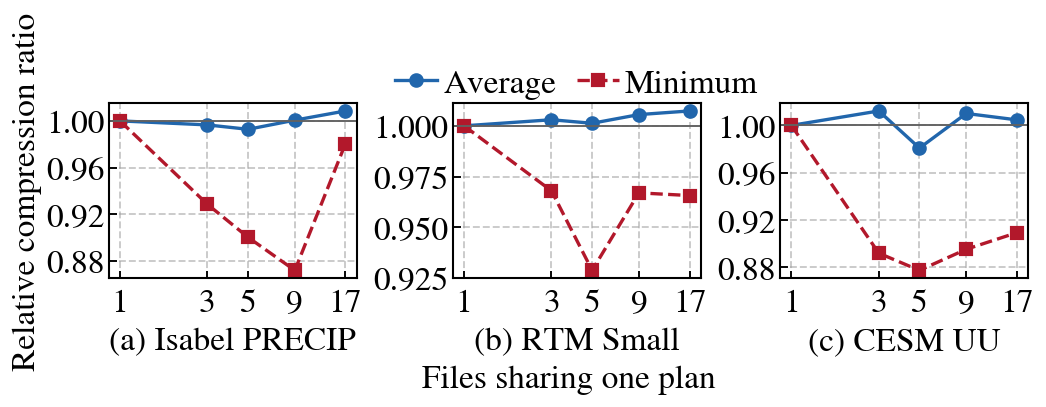
\includegraphics{revised-fig/temporal-plan-reuse.png}
    \caption{Relative compression ratio of temporal plan reuse at matched PSNR. Each panel plots the average over the evaluated files and the minimum over individual files against the number of files that share one plan. A value of 1 means that the transferred plan matches the self-generated plan.}
    \label{fig:evaluation-temporal-reuse}
\end{figure}

\subsubsection{Reuse Across Non-Temporal Related Arrays}

The non-temporal experiments transfer plans across arrays that come from the same application but differ in orbital index, velocity component, or number of frames. Figure~\ref{fig:evaluation-non-temporal-reuse} shows that transferability depends on how similar the arrays are. Neighboring QMCPACK orbitals, the two horizontal Isabel wind components, and the two APSU datasets at fine error bounds exchange plans with little loss, whereas the vertical and horizontal wind components require separate plans.

QMCPACK orbitals 0--287 share the same $115\times69\times69$ spline grid and include QMCPACK orbital 144 from the 18 evaluated fields. We order the orbitals by index and apply the windows defined above with $m\in\{1,3,5,9,17\}$. The average relative compression ratio stays between 0.98 and 0.99 for every $m>1$, but individual orbitals vary more than consecutive snapshots. Six orbitals select 1D4R at $10^{-3}$, and all other orbitals select 1D6R. At $m=3$ and $m=5$, the lowest ratios, 0.63 and 0.67, occur when one of these six orbitals generates the plan for neighbors that select 1D6R. None of these orbitals generates a plan at $m=9$ or $m=17$, and the minimum rises to 0.81 and 0.83, respectively.

Isabel time step 24 provides the wind components U, V, and W on the same $100\times500\times500$ grid, and we apply the plan of each component to the other two. U and V exchange plans with relative compression ratios of 0.99 and 1.00. Plans transferred between W and either horizontal component reach only 0.46 to 0.64. In its two finest rounds, the W plan predicts along the vertical axis, whereas the U and V plans predict along horizontal axes. These two rounds contain about three quarters of all targets, so this difference dominates the compression ratio.

APSU 004 and APSU 006 contain 1024 and 4096 frames, respectively, from the same $1558\times1813$ X-ray detector. We generate the plans on the smaller APSU 004 and apply them to APSU 006, which removes the 102 to 132~s of plan generation on APSU 006. Because this experiment has a single target file, we compute the relative compression ratio at the PSNR of the self-generated plan at each of the five evaluated error bounds. The ratio is at least 0.99 at $10^{-3}$ and finer bounds and decreases to 0.91 at $10^{-2}$ and 0.64 at $10^{-1}$. Plans transferred from the smaller dataset therefore suit APSU 006 from the middle error bound to the finest bound, while the two coarsest bounds benefit from a plan generated on APSU 006 itself.

\begin{figure}[htb]
    \centering
    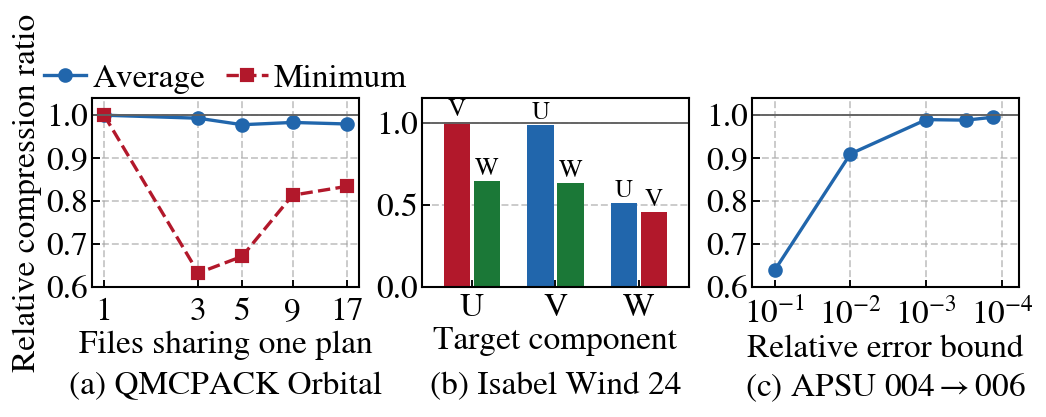
\includegraphics{revised-fig/non-temporal-plan-reuse.png}
    \caption{Relative compression ratio of non-temporal plan reuse at matched PSNR. (a) Average and minimum over QMCPACK orbitals against the number of orbitals that share one plan. (b) Ratio for each Isabel wind component under the plans of the other two components, labeled above each bar. (c) Ratio for APSU 006 under the APSU 004 plan at each error bound. A value of 1 means that the transferred plan matches the self-generated plan.}
    \label{fig:evaluation-non-temporal-reuse}
\end{figure}
